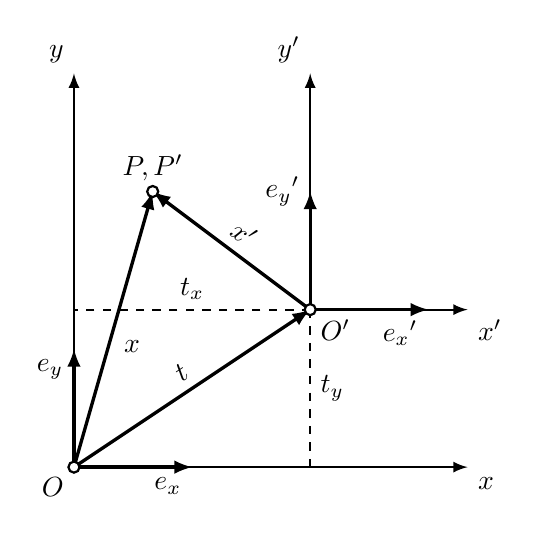
\begin{tikzpicture}
    %\sansmath
    %----------------------------------------------------------------------------------------%
    % Koordinaten
    %----------------------------------------------------------------------------------------%
    \coordinate (O1) at (0,0);
    \coordinate (O2) at (3,2);
    \coordinate (P) at (1,3.5);
    %----------------------------------------------------------------------------------------%
    % Koordinatenachsen
    %----------------------------------------------------------------------------------------%
    \begin{scope}[thick,->,>=latex]
    \draw (O1) -- +(5,0) node[anchor=north west] {$x$};
    \draw (O1) -- +(0,5) node[anchor=south east] {$y$};
    \end{scope}
    \begin{scope}[thick,->,>=latex]
    \draw (O2) -- +(2,0) node[anchor=north west] {$x^\prime$};
    \draw (O2) -- +(0,3) node[anchor=south east] {$y^\prime$};
    \end{scope}
    %----------------------------------------------------------------------------------------%
    % Einheitsvektoren
    %----------------------------------------------------------------------------------------%
    \begin{scope}[very thick,->,>=latex,scale=1.5]
    \draw (O1) -- +(1,0) node[anchor=north east] {$\bvec{e_{x}}$};
    \draw (O1) -- +(0,1) node[anchor=north east] {$\bvec{e_{y}}$};
    \draw (O2) -- +(1,0) node[anchor=north east] {$\bvec{e_{x}}^\prime$};
    \draw (O2) -- +(0,1) node[anchor=east] {$\bvec{e_{y}}^\prime$};
    \end{scope}
    %----------------------------------------------------------------------------------------%
    % Vektoren
    %----------------------------------------------------------------------------------------%
    \begin{scope}[very thick,->,>=latex]
    \draw (O1) -- (P) node [midway, anchor = north west] {$\bvec{x}$};
    \draw (O2) -- (P) node [midway, sloped, above] {$\bvec{x}^\prime$};
    \draw (O1) -- (O2) node [midway, sloped, above] {$\bvec{t}$};
    \end{scope}
    %----------------------------------------------------------------------------------------%
    % Komponenten
    %----------------------------------------------------------------------------------------%
    \begin{scope}[thick, dashed]
    \draw (O2) -- (O1|-O2) node [midway, above] {$t_{x}$};
    \draw (O2) -- (O1-|O2) node [midway, anchor = west] {$t_{y}$};
    \end{scope}
    %----------------------------------------------------------------------------------------%
    % Punkte
    %----------------------------------------------------------------------------------------%
    \begin{scope}[thick,draw=black,fill=white]
    \filldraw (O1) circle (2pt) node[anchor=north east] {$O$};
    \filldraw (O2) circle (2pt) node[anchor=north west] {$O^\prime$};
    \filldraw (P) circle (2pt) node[anchor=south] {$P,P^\prime$};
    \end{scope}
\end{tikzpicture}